\documentclass{report}
\usepackage{blindtext}
\usepackage{hyperref}
\usepackage[pdftex]{graphicx}
\usepackage[T1]{fontenc}
\usepackage{color}
\usepackage{varioref}
\usepackage{textcomp}
\usepackage{amsthm}
\usepackage{amsmath}
\usepackage{amssymb}
\usepackage{graphicx}
\usepackage{setspace}
\usepackage{esint}
\usepackage{algorithm}
\usepackage{algpseudocode}
\usepackage{pifont}
\usepackage{amsmath}
\usepackage{amsmath,bm}
\usepackage{enumitem}
\usepackage{xcolor}
\usepackage{amsmath}
\usepackage{tcolorbox}
\usepackage{hyperref}
\usepackage{tikz}
\usepackage[margin=3cm]{geometry} % Adjust margins here


\hypersetup{
    colorlinks=true,
    linkcolor=black,
    filecolor=magenta,      
    urlcolor=cyan,
    pdftitle={Linear Algebra},
    pdfpagemode=FullScreen,
    }
\begin{document}

\tableofcontents
\clearpage

% Pop quiz for linear problems.
%%%%%%%%%%%%% FIRST SECTION
% \section{Matrix Operations}

%%%%%%%%%%%%%%%%%%%%%%%%%%%%%%%%%%%%%%%%%%%%%%%%%%%%%%%%%%%%%%%%
%%%%%EXAMPLE
% \begin{tcolorbox}[colback=gray!10, boxrule=0pt]
% \textbf{EXAMPLE TEMPLATE}
% Perform matrix addition for the following matrices:
% \[
% A = \begin{bmatrix}
% 2 & 3 \\
% -1 & 4
% \end{bmatrix}
% \quad \text{and} \quad
% B = \begin{bmatrix}
% 5 & -2 \\
% 0 & 1
% \end{bmatrix}
% \]

% To add two matrices, simply add the corresponding elements:
% \[
% A + B = \begin{bmatrix}
% 2 + 5 & 3 + (-2) \\
% (-1) + 0 & 4 + 1
% \end{bmatrix}
% \]

% Performing the addition:
% \[
% A + B = \begin{bmatrix}
% 7 & 1 \\
% -1 & 5
% \end{bmatrix}
% \]

% So, the sum of matrices \(A\) and \(B\) is:
% \[
% A + B = \begin{bmatrix}
% 7 & 1 \\
% -1 & 5
% \end{bmatrix}
% \]
% \end{tcolorbox}


%%%%%%%%%%%%%%%%%%%%%%%%%%%%%%% MATRIX DEFENITION
\section{Matrix Definitions and Operations}
\noindent \textbf{Definition 1.1} (Matrix).
A real-valued $(m, n)$ matrix $A$ with $m, n \in \mathbb{N}$ is an $m \cdot n$-tuple of elements $a_{ij}$, where $i = 1, \ldots, m$ and $j = 1, \ldots, n$, arranged in a rectangular pattern with $m$ rows and $n$ columns:

\[ A = \begin{bmatrix} 
a_{11} & a_{12} & \cdots & a_{1n} \\
a_{21} & a_{22} & \cdots & a_{2n} \\
\vdots & \vdots & \ddots & \vdots \\
a_{m1} & a_{m2} & \cdots & a_{mn} 
\end{bmatrix} \]
\\
%%%%%%%%%%%%%%%%%%%%%%%%%%%%%%% MATRIX ADDITION
\noindent
Matrix addition is an operation performed on two matrices of the same size. Given matrices $A \in \mathbb{R}^{m\times n}$ and $B \in \mathbb{R}^{m\times n}$, adding the matrices together involves adding their corresponding elements (Element-Wise):


\[ A + B = \begin{bmatrix}
a_{11} + b_{11} & a_{12} + b_{12} & \cdots & a_{1n} + b_{1n} \\
a_{21} + b_{21} & a_{22} + b_{22} & \cdots & a_{2n} + b_{2n} \\
\vdots & \vdots & \ddots & \vdots \\
a_{m1} + b_{m1} & a_{m2} + b_{m2} & \cdots & a_{mn} + b_{mn}
\end{bmatrix} \]


%%%%%%%%%%%%%%%%%%%%%%%%%%%%%%% MATRIX MULTIPLICATION
\noindent Matrix multiplication is performed between two matrices, $A \in \mathbb{R}^{m\times n}$, $B \in \mathbb{R}^{n \times k}$, and results in $C = AB \in \mathbb{R}^{m \times k}$. The product \( C \) is calculated by taking the dot product of each row of matrix \( A \) with each column of matrix \( B \). We sum the products of the multiplication to obtain an entry in the corresponding row $i$ and column $j$ of C.

\[ c_{ij} = \sum_{k=1}^{n} a_{ik} \cdot b_{kj} \] 
\begin{itemize}
    \item $a_{ik}$ is the element at row $i$ and column $k$ of matrix $A$,
    \item $b_{kj}$ is the element at row $k$ and column $j$ of matrix $B$,
    \item $n$ is the number of columns in matrix $A$ (which is also the number of rows in matrix $B$).
\end{itemize}
such that

\[ A = \begin{bmatrix} 
a_{11} & a_{12} \\
a_{21} & a_{22} \\
a_{31} & a_{32} \\
\end{bmatrix} \in \mathbb{R}^{3 \times 2}, \quad
B = \begin{bmatrix} 
b_{11} & b_{12} & b_{13} \\
b_{21} & b_{22} & b_{23} \\
\end{bmatrix} \in \mathbb{R}^{2 \times 3}\]

\[ C = \begin{bmatrix} 
a_{11}b_{11} + a_{12}b_{21} & a_{11}b_{12} + a_{12}b_{22} & a_{11}b_{13} + a_{12}b_{23} \\
a_{21}b_{11} + a_{22}b_{21} & a_{21}b_{12} + a_{22}b_{22} & a_{21}b_{13} + a_{22}b_{23} \\
a_{31}b_{11} + a_{32}b_{21} & a_{31}b_{12} + a_{32}b_{22} & a_{31}b_{13} + a_{32}b_{23} \\
\end{bmatrix} \]

%%%%%%%%%%%%%%%%%%%% IDENTITY
\noindent \textbf{Definition 1.2} (Identity Matrix).
A matrix in $\mathbb{R}^{n \times n}$ that contains only 1's on its diagonal entries. 

\[ I_n := \begin{bmatrix} 
1 & 0 & \cdots & 0 \\
0 & 1 & \cdots & 0 \\
\vdots & \vdots & \ddots & \vdots \\
0 & 0 & \cdots & 1
\end{bmatrix} \]


%%%%%%%%%%%%%%%%%%%%% Linear Independence
\newpage
\noindent \textbf{Definition 1.3} (Linear Independence).
In a linearly independent matrix, each column holds the property that it cannot be expressed by performing linear combinations of the other columns. i.e. if a matrix has 3 columns, you cannot multiply columns 2 or 3 by any value $c \in \mathbb{R}$ such that the columns would be the same as column 1 and vice versa. It also holds that adding two columns together with the ability to scale them also cannot equal another column in the matrix. \\
The formal definition states: 
A set of vectors \( \{ \mathbf{v}_1, \mathbf{v}_2, \ldots, \mathbf{v}_n \} \) in a vector space \( V \) over a field \( F \) is said to be linearly independent if the only scalars \( c_1, c_2, \ldots, c_n \) satisfying the equation

\[ c_1 \mathbf{v}_1 + c_2 \mathbf{v}_2 + \ldots + c_n \mathbf{v}_n = \mathbf{0} \]

the only solution to this should be \( c_1 = c_2 = \ldots = c_n = 0 \). In other words, the only way to obtain the zero vector \( \mathbf{0} \) as a linear combination of the vectors \( \mathbf{v}_1, \mathbf{v}_2, \ldots, \mathbf{v}_n \) is by setting all the scalar coefficients to zero.

\section{3D Vector Space Representation}

\begin{figure}[h]
    \centering
    \begin{tikzpicture}[scale=1.5]
        % Axes
        \draw[thick,->] (0,0,0) -- (2,0,0) node[anchor=north east]{$y$};
        \draw[thick,->] (0,0,0) -- (0,2,0) node[anchor=north west]{$z$};
        \draw[thick,->] (0,0,0) -- (0,0,2) node[anchor=south]{$x$};
        % Origin
        \filldraw[black] (0,0,0) circle (0.05) node[anchor=north west]{$0$};
        % Vector
        \draw[thick,->] (0,0,0) -- (1.5,1.5,1) node[anchor=west]{$\mathbf{U}$};
    \end{tikzpicture}
    \caption{A vector in three-dimensional space. Starting at fixed point 0, the vector v represents the point $\mathbf{U}$.}
    \label{fig:vector_diagram}
\end{figure}

%%%%%%%%%%%%%%%%%%%%% EXAMPLE FIGURE
\begin{figure}[h]
    \begin{tcolorbox}[colback=gray!10, boxrule=0pt] 
    \textbf{EXAMPLE} \\
    \\
        \centering
        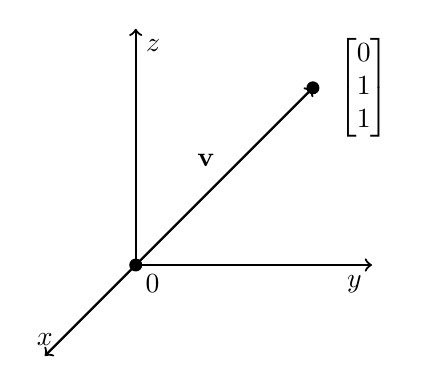
\begin{tikzpicture}[scale=1.5]
            % Axes
            \draw[thick,->] (0,0) -- (2,0) node[anchor=north east]{$y$};
            \draw[thick,->] (0,0) -- (0,2) node[anchor=north west]{$z$};
            \draw[thick,->] (0,0,0) -- (0,0,2) node[anchor=south]{$x$};
            % Origin
            \filldraw[black] (0,0) circle (0.05) node[anchor=north west]{$0$};
            % Vector
            \draw[thick,->] (0,0) -- (1.5,1.5) node[anchor=west]{};
            % Label for the vector
            \node[anchor=south east] at (0.75,0.75) {$\mathbf{v}$};
            % Point P
            \filldraw[black] (1.5,1.5) circle (0.05) node[anchor=west, xshift=2mm]{
                $\begin{bmatrix} 
                0 \\
                1 \\
                1
                \end{bmatrix}$
            };
        \end{tikzpicture}
        \label{fig:vector_point}

    Notice that the 1st value in the vector (representing x), $v \in \mathbb{R}$ is 0 so the vector stays on the z and y axis.
    \end{tcolorbox}
\end{figure}

%%%%%%%%%%%%%%%%%%%%% Commutative Property
\noindent \textbf{Definition 1.3} (Commutative Property).
Matrix multiplication is not commutative. For Arithmetic operations of matrices, the commutative property is applied to $A + B = B + A$ as it would be applied to $5 + 7 = 7 + 5$. This is illustrated by the following example
%%%%%EXAMPLE
\begin{tcolorbox}[colback=gray!10, boxrule=0pt]
    \textbf{EXAMPLE}
    Perform matrix addition for the following matrices:
    \[
    A = \begin{bmatrix}
    2 & 3 \\
    -1 & 4
    \end{bmatrix}
    \quad \text{and} \quad
    B = \begin{bmatrix}
    5 & -2 \\
    0 & 1
    \end{bmatrix}
    \]
    
    To add two matrices, simply add the corresponding elements:
    \[
    A + B = \begin{bmatrix}
    2 + 5 & 3 + (-2) \\
    (-1) + 0 & 4 + 1
    \end{bmatrix}
    = \begin{bmatrix}
    7 & 1 \\
    -1 & 5
    \end{bmatrix}
    \]
    
    By the commutative property:
    \[
    B + A = \begin{bmatrix}
    5 + 2 & (-2) + 3 \\
    0 + (-1) & 1 + 4
    \end{bmatrix}
    =  \begin{bmatrix}
    7 & 1 \\
    -1 & 5
    \end{bmatrix}
    \]
    
    So, the sum of matrices \(A\) and \(B\) is:
    \[
    A + B = \begin{bmatrix}
    7 & 1 \\
    -1 & 5
    \end{bmatrix} = B + A
    \]
\end{tcolorbox}
\noindent This example demonstrates the commutative property in 2-dimensions. The same property applies to tensors, where the difference is that the addition is performed on multiple matrices, not just 2. In quantum computing, operations on qubits are represented by matrices called quantum gates. 

\section{Tensors}
\textbf{Definition 1.4} (Tensors) A Tensor is a multidimensional array. Image a matrix like a flat sheet of paper, and a tensor is when you stack more than 1 onto it.\\

\noindent Kronecker product of two tensors
\begin{align}
    T_1 \otimes T_2 = \begin{bmatrix}
    t_{11} \cdot T_2 & t_{12} \cdot T_2 & \cdots & t_{1n} \cdot T_2 \\
    t_{21} \cdot T_2 & t_{22} \cdot T_2 & \cdots & t_{2n} \cdot T_2 \\
    \vdots & \vdots & \ddots & \vdots \\
    t_{m1} \cdot T_2 & t_{m2} \cdot T_2 & \cdots & t_{mn} \cdot T_2
\end{bmatrix}
\end{align}
% Commutative property of Kronecker product
$T_1 \otimes T_2$ = $T_2 \otimes T_1$
\section{}

\end{document}
